\documentclass[twoside]{book}

% Packages required by doxygen
\usepackage{fixltx2e}
\usepackage{calc}
\usepackage{doxygen}
\usepackage[export]{adjustbox} % also loads graphicx
\usepackage{graphicx}
\usepackage[utf8]{inputenc}
\usepackage{makeidx}
\usepackage{multicol}
\usepackage{multirow}
\PassOptionsToPackage{warn}{textcomp}
\usepackage{textcomp}
\usepackage[nointegrals]{wasysym}
\usepackage[table]{xcolor}

% Font selection
\usepackage[T1]{fontenc}
\usepackage[scaled=.90]{helvet}
\usepackage{courier}
\usepackage{amssymb}
\usepackage{sectsty}
\renewcommand{\familydefault}{\sfdefault}
\allsectionsfont{%
  \fontseries{bc}\selectfont%
  \color{darkgray}%
}
\renewcommand{\DoxyLabelFont}{%
  \fontseries{bc}\selectfont%
  \color{darkgray}%
}
\newcommand{\+}{\discretionary{\mbox{\scriptsize$\hookleftarrow$}}{}{}}

% Page & text layout
\usepackage{geometry}
\geometry{%
  a4paper,%
  top=2.5cm,%
  bottom=2.5cm,%
  left=2.5cm,%
  right=2.5cm%
}
\tolerance=750
\hfuzz=15pt
\hbadness=750
\setlength{\emergencystretch}{15pt}
\setlength{\parindent}{0cm}
\setlength{\parskip}{3ex plus 2ex minus 2ex}
\makeatletter
\renewcommand{\paragraph}{%
  \@startsection{paragraph}{4}{0ex}{-1.0ex}{1.0ex}{%
    \normalfont\normalsize\bfseries\SS@parafont%
  }%
}
\renewcommand{\subparagraph}{%
  \@startsection{subparagraph}{5}{0ex}{-1.0ex}{1.0ex}{%
    \normalfont\normalsize\bfseries\SS@subparafont%
  }%
}
\makeatother

% Headers & footers
\usepackage{fancyhdr}
\pagestyle{fancyplain}
\fancyhead[LE]{\fancyplain{}{\bfseries\thepage}}
\fancyhead[CE]{\fancyplain{}{}}
\fancyhead[RE]{\fancyplain{}{\bfseries\leftmark}}
\fancyhead[LO]{\fancyplain{}{\bfseries\rightmark}}
\fancyhead[CO]{\fancyplain{}{}}
\fancyhead[RO]{\fancyplain{}{\bfseries\thepage}}
\fancyfoot[LE]{\fancyplain{}{}}
\fancyfoot[CE]{\fancyplain{}{}}
\fancyfoot[RE]{\fancyplain{}{\bfseries\scriptsize Generated by Doxygen }}
\fancyfoot[LO]{\fancyplain{}{\bfseries\scriptsize Generated by Doxygen }}
\fancyfoot[CO]{\fancyplain{}{}}
\fancyfoot[RO]{\fancyplain{}{}}
\renewcommand{\footrulewidth}{0.4pt}
\renewcommand{\chaptermark}[1]{%
  \markboth{#1}{}%
}
\renewcommand{\sectionmark}[1]{%
  \markright{\thesection\ #1}%
}

% Indices & bibliography
\usepackage{natbib}
\usepackage[titles]{tocloft}
\setcounter{tocdepth}{3}
\setcounter{secnumdepth}{5}
\makeindex

% Hyperlinks (required, but should be loaded last)
\usepackage{ifpdf}
\ifpdf
  \usepackage[pdftex,pagebackref=true]{hyperref}
\else
  \usepackage[ps2pdf,pagebackref=true]{hyperref}
\fi
\hypersetup{%
  colorlinks=true,%
  linkcolor=blue,%
  citecolor=blue,%
  unicode%
}

% Custom commands
\newcommand{\clearemptydoublepage}{%
  \newpage{\pagestyle{empty}\cleardoublepage}%
}

\usepackage{caption}
\captionsetup{labelsep=space,justification=centering,font={bf},singlelinecheck=off,skip=4pt,position=top}

%===== C O N T E N T S =====

\begin{document}

% Titlepage & ToC
\hypersetup{pageanchor=false,
             bookmarksnumbered=true,
             pdfencoding=unicode
            }
\pagenumbering{alph}
\begin{titlepage}
\vspace*{7cm}
\begin{center}%
{\Large MngX }\\
\vspace*{1cm}
{\large Generated by Doxygen 1.8.14}\\
\end{center}
\end{titlepage}
\clearemptydoublepage
\pagenumbering{roman}
\tableofcontents
\clearemptydoublepage
\pagenumbering{arabic}
\hypersetup{pageanchor=true}

%--- Begin generated contents ---
\chapter{Hierarchical Index}
\section{Class Hierarchy}
This inheritance list is sorted roughly, but not completely, alphabetically\+:\begin{DoxyCompactList}
\item \contentsline{section}{Config}{\pageref{class_config}}{}
\item \contentsline{section}{Control}{\pageref{class_control}}{}
\item \contentsline{section}{Directory}{\pageref{class_directory}}{}
\begin{DoxyCompactList}
\item \contentsline{section}{Config\+\_\+\+Directory}{\pageref{class_config___directory}}{}
\item \contentsline{section}{Directory\+\_\+\+Structure}{\pageref{class_directory___structure}}{}
\end{DoxyCompactList}
\item \contentsline{section}{Interface}{\pageref{class_interface}}{}
\item Q\+Main\+Window\begin{DoxyCompactList}
\item \contentsline{section}{Main\+Window}{\pageref{class_main_window}}{}
\end{DoxyCompactList}
\end{DoxyCompactList}

\chapter{Class Index}
\section{Class List}
Here are the classes, structs, unions and interfaces with brief descriptions\+:\begin{DoxyCompactList}
\item\contentsline{section}{\mbox{\hyperlink{class_config}{Config}} \\*Manage config files }{\pageref{class_config}}{}
\item\contentsline{section}{\mbox{\hyperlink{class_config___directory}{Config\+\_\+\+Directory}} }{\pageref{class_config___directory}}{}
\item\contentsline{section}{\mbox{\hyperlink{class_control}{Control}} \\*Input and control flow managment }{\pageref{class_control}}{}
\item\contentsline{section}{\mbox{\hyperlink{class_directory}{Directory}} \\*Manage directory and path }{\pageref{class_directory}}{}
\item\contentsline{section}{\mbox{\hyperlink{class_directory___structure}{Directory\+\_\+\+Structure}} }{\pageref{class_directory___structure}}{}
\item\contentsline{section}{\mbox{\hyperlink{class_interface}{Interface}} }{\pageref{class_interface}}{}
\item\contentsline{section}{\mbox{\hyperlink{class_main_window}{Main\+Window}} }{\pageref{class_main_window}}{}
\end{DoxyCompactList}

\chapter{Class Documentation}
\hypertarget{class_config}{}\section{Config Class Reference}
\label{class_config}\index{Config@{Config}}


Manage config files.  




{\ttfamily \#include $<$config.\+h$>$}

\subsection*{Public Types}
\begin{DoxyCompactItemize}
\item 
\mbox{\Hypertarget{class_config_aecaa9226d0d87955e3813b7e12da5bd3}\label{class_config_aecaa9226d0d87955e3813b7e12da5bd3}} 
enum {\bfseries S\+E\+C\+T\+I\+ON} \{ {\bfseries G\+L\+O\+B\+AL} = 0, 
{\bfseries M\+A\+J\+OR} = 1, 
{\bfseries S\+U\+B\+\_\+\+C\+O\+N\+F\+IG} = 2
 \}
\end{DoxyCompactItemize}
\subsection*{Public Member Functions}
\begin{DoxyCompactItemize}
\item 
\mbox{\Hypertarget{class_config_ad74e2a92db53fa68dadf2efd0d8b59be}\label{class_config_ad74e2a92db53fa68dadf2efd0d8b59be}} 
{\bfseries Config} (const std\+::string \&)
\item 
\mbox{\Hypertarget{class_config_a7467670e36e879accebd5ede185724c9}\label{class_config_a7467670e36e879accebd5ede185724c9}} 
\mbox{\hyperlink{class_config}{Config}} \& {\bfseries operator=} (const \mbox{\hyperlink{class_config}{Config}} \&)
\item 
\mbox{\Hypertarget{class_config_a6fb87004fcddb63a908a5e27f70dc014}\label{class_config_a6fb87004fcddb63a908a5e27f70dc014}} 
\mbox{\hyperlink{class_config}{Config}} \& {\bfseries operator=} (const std\+::string \&)
\item 
\mbox{\Hypertarget{class_config_aef0ec22ee92ab7f39647cd22ec34e0e4}\label{class_config_aef0ec22ee92ab7f39647cd22ec34e0e4}} 
void \mbox{\hyperlink{class_config_aef0ec22ee92ab7f39647cd22ec34e0e4}{creat}} ()
\begin{DoxyCompactList}\small\item\em create config file in assignment path \end{DoxyCompactList}\item 
\mbox{\Hypertarget{class_config_aee780600cc3fb3ad239730e113379436}\label{class_config_aee780600cc3fb3ad239730e113379436}} 
void \mbox{\hyperlink{class_config_aee780600cc3fb3ad239730e113379436}{creat}} (const std\+::string \&)
\begin{DoxyCompactList}\small\item\em asssing path and creat config file \end{DoxyCompactList}\item 
\mbox{\Hypertarget{class_config_a5e31b9666527f099f1a542d4ec668e40}\label{class_config_a5e31b9666527f099f1a542d4ec668e40}} 
bool \mbox{\hyperlink{class_config_a5e31b9666527f099f1a542d4ec668e40}{add\+\_\+row}} (const S\+E\+C\+T\+I\+ON, const std\+::string \&)
\begin{DoxyCompactList}\small\item\em add one row in config file section \end{DoxyCompactList}\item 
\mbox{\Hypertarget{class_config_a9db2df151d53943ec0c02358cdc6c8e0}\label{class_config_a9db2df151d53943ec0c02358cdc6c8e0}} 
bool \mbox{\hyperlink{class_config_a9db2df151d53943ec0c02358cdc6c8e0}{remove\+\_\+row}} (const S\+E\+C\+T\+I\+ON, const std\+::string \&)
\begin{DoxyCompactList}\small\item\em remove one row in config file section \end{DoxyCompactList}\item 
\mbox{\Hypertarget{class_config_a6f868d196b3590d940e91e31c98ab85b}\label{class_config_a6f868d196b3590d940e91e31c98ab85b}} 
string\+\_\+vec \mbox{\hyperlink{class_config_a6f868d196b3590d940e91e31c98ab85b}{get\+\_\+section}} (const S\+E\+C\+T\+I\+ON)
\begin{DoxyCompactList}\small\item\em return section content from section \end{DoxyCompactList}\item 
\mbox{\Hypertarget{class_config_a4d4698876d10131043806b0ddd690eb3}\label{class_config_a4d4698876d10131043806b0ddd690eb3}} 
void \mbox{\hyperlink{class_config_a4d4698876d10131043806b0ddd690eb3}{clear}} ()
\begin{DoxyCompactList}\small\item\em clear assignment path \end{DoxyCompactList}\item 
\mbox{\Hypertarget{class_config_a170d9cc2b65ee82abcf7f1ed91e7ee5c}\label{class_config_a170d9cc2b65ee82abcf7f1ed91e7ee5c}} 
bool \mbox{\hyperlink{class_config_a170d9cc2b65ee82abcf7f1ed91e7ee5c}{status}} () const
\begin{DoxyCompactList}\small\item\em return file.\+name.\+empty() \end{DoxyCompactList}\end{DoxyCompactItemize}


\subsection{Detailed Description}
Manage config files. 

\mbox{\hyperlink{class_config}{Config}} class should be initialize with path to config file. For default path use a take\+\_\+default\+\_\+path() from a object of \mbox{\hyperlink{class_config___directory}{Config\+\_\+\+Directory}} class. 

The documentation for this class was generated from the following files\+:\begin{DoxyCompactItemize}
\item 
include/config.\+h\item 
src/config.\+cpp\end{DoxyCompactItemize}

\hypertarget{class_config___directory}{}\section{Config\+\_\+\+Directory Class Reference}
\label{class_config___directory}\index{Config\+\_\+\+Directory@{Config\+\_\+\+Directory}}
Inheritance diagram for Config\+\_\+\+Directory\+:\begin{figure}[H]
\begin{center}
\leavevmode
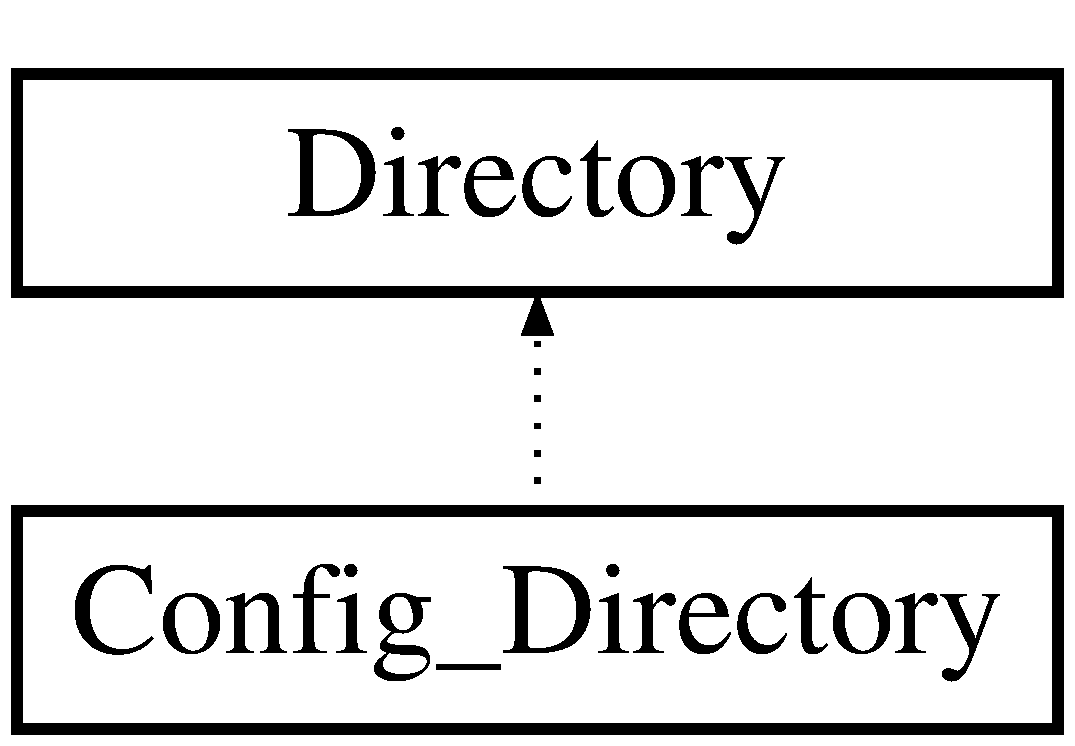
\includegraphics[height=2.000000cm]{class_config___directory}
\end{center}
\end{figure}
\subsection*{Public Member Functions}
\begin{DoxyCompactItemize}
\item 
\mbox{\Hypertarget{class_config___directory_ae51312baad8bbef3b29ab7a592b7e12f}\label{class_config___directory_ae51312baad8bbef3b29ab7a592b7e12f}} 
std\+::string {\bfseries take\+\_\+default\+\_\+path} ()
\end{DoxyCompactItemize}


The documentation for this class was generated from the following files\+:\begin{DoxyCompactItemize}
\item 
include/config\+\_\+directory.\+h\item 
src/config\+\_\+directory.\+cpp\end{DoxyCompactItemize}

\hypertarget{class_control}{}\section{Control Class Reference}
\label{class_control}\index{Control@{Control}}


Input and control flow managment.  




{\ttfamily \#include $<$control.\+h$>$}

\subsection*{Public Types}
\begin{DoxyCompactItemize}
\item 
\mbox{\Hypertarget{class_control_a611d69b6e2dd463089387b8ef867e939}\label{class_control_a611d69b6e2dd463089387b8ef867e939}} 
enum {\bfseries C\+O\+M\+M\+A\+N\+D\+\_\+\+F\+L\+AG} \{ \newline
{\bfseries U\+N\+K\+N\+O\+W\+N\+\_\+\+C\+O\+M\+M\+A\+ND} = 0, 
{\bfseries H\+E\+LP} = 1, 
{\bfseries C\+O\+N\+F\+IG} = 2, 
{\bfseries C\+R\+E\+AT} = 100, 
\newline
{\bfseries L\+O\+AD} = 101, 
{\bfseries A\+D\+D\+\_\+\+D\+I\+R\+E\+C\+T\+O\+RY} = 102, 
{\bfseries R\+E\+M\+O\+V\+E\+\_\+\+D\+I\+R\+E\+C\+T\+O\+RY} = 103
 \}
\end{DoxyCompactItemize}
\subsection*{Public Member Functions}
\begin{DoxyCompactItemize}
\item 
\mbox{\Hypertarget{class_control_a3201b6907d22e4034c0eceaf38d78449}\label{class_control_a3201b6907d22e4034c0eceaf38d78449}} 
\mbox{\hyperlink{class_control_a3201b6907d22e4034c0eceaf38d78449}{Control}} (const int, char $\ast$$\ast$)
\begin{DoxyCompactList}\small\item\em manage input from stdin \end{DoxyCompactList}\item 
\mbox{\Hypertarget{class_control_a8cc17820380c76b49979134fb2bb0280}\label{class_control_a8cc17820380c76b49979134fb2bb0280}} 
{\bfseries Control} (const std\+::string \&)
\item 
\mbox{\Hypertarget{class_control_a2c2cb5a17c8a125350c543097b188f67}\label{class_control_a2c2cb5a17c8a125350c543097b188f67}} 
{\bfseries Control} (const \mbox{\hyperlink{class_control}{Control}} \&)
\item 
\mbox{\Hypertarget{class_control_a84586bbffaee27751ae8a4004c1f3a5e}\label{class_control_a84586bbffaee27751ae8a4004c1f3a5e}} 
\mbox{\hyperlink{class_control}{Control}} \& {\bfseries operator=} (const \mbox{\hyperlink{class_control}{Control}} \&)
\item 
\mbox{\Hypertarget{class_control_af158514e9f3c5bdd6a31ec409d48dc3b}\label{class_control_af158514e9f3c5bdd6a31ec409d48dc3b}} 
\mbox{\hyperlink{class_control}{Control}} \& {\bfseries operator=} (const std\+::string \&)
\item 
\mbox{\Hypertarget{class_control_a65c77a675ccc4a39476354cf1222419a}\label{class_control_a65c77a675ccc4a39476354cf1222419a}} 
\mbox{\hyperlink{class_control}{Control}} \& \mbox{\hyperlink{class_control_a65c77a675ccc4a39476354cf1222419a}{operator+=}} (const \mbox{\hyperlink{class_control}{Control}} \&)
\begin{DoxyCompactList}\small\item\em add commands and incorrect\+\_\+flags \end{DoxyCompactList}\item 
\mbox{\Hypertarget{class_control_aacf7ffe575257d1fb7a8183e53881fb8}\label{class_control_aacf7ffe575257d1fb7a8183e53881fb8}} 
\mbox{\hyperlink{class_control}{Control}} \& \mbox{\hyperlink{class_control_aacf7ffe575257d1fb7a8183e53881fb8}{operator+=}} (const std\+::string \&)
\begin{DoxyCompactList}\small\item\em add commands and incorrect\+\_\+flags \end{DoxyCompactList}\item 
\mbox{\Hypertarget{class_control_a17fc1437bd16b3c299b2c9d24e69e4e6}\label{class_control_a17fc1437bd16b3c299b2c9d24e69e4e6}} 
bool \mbox{\hyperlink{class_control_a17fc1437bd16b3c299b2c9d24e69e4e6}{set\+\_\+argv}} (const int, char $\ast$$\ast$)
\begin{DoxyCompactList}\small\item\em manage input from stdin \end{DoxyCompactList}\item 
\mbox{\Hypertarget{class_control_a6292968ec14391686b392a66dd8c7029}\label{class_control_a6292968ec14391686b392a66dd8c7029}} 
bool {\bfseries set\+\_\+input} (const std\+::string \&)
\item 
\mbox{\Hypertarget{class_control_abf673cb93f661b8b044c1c7f3f627a77}\label{class_control_abf673cb93f661b8b044c1c7f3f627a77}} 
std\+::string \mbox{\hyperlink{class_control_abf673cb93f661b8b044c1c7f3f627a77}{get\+\_\+incorrect\+\_\+flag}} ()
\begin{DoxyCompactList}\small\item\em return front and pop\+\_\+front \end{DoxyCompactList}\item 
\mbox{\Hypertarget{class_control_abd01cc233279071e4425c31a6a394bcf}\label{class_control_abd01cc233279071e4425c31a6a394bcf}} 
bool \mbox{\hyperlink{class_control_abd01cc233279071e4425c31a6a394bcf}{status}} () const
\begin{DoxyCompactList}\small\item\em return incorrect\+\_\+flags.\+empty(); \end{DoxyCompactList}\item 
\mbox{\Hypertarget{class_control_a12a2da2687aee8950d75060225ae5a7a}\label{class_control_a12a2da2687aee8950d75060225ae5a7a}} 
bool \mbox{\hyperlink{class_control_a12a2da2687aee8950d75060225ae5a7a}{empty}} () const
\begin{DoxyCompactList}\small\item\em return commands.\+empty(); \end{DoxyCompactList}\item 
\mbox{\Hypertarget{class_control_a61a69b63095c78c8de94e83a1e72a1a6}\label{class_control_a61a69b63095c78c8de94e83a1e72a1a6}} 
void \mbox{\hyperlink{class_control_a61a69b63095c78c8de94e83a1e72a1a6}{clear}} ()
\begin{DoxyCompactList}\small\item\em clear commands and incorrect\+\_\+flags \end{DoxyCompactList}\item 
\mbox{\Hypertarget{class_control_a3ce5920b84869542d1b5bca6ea925abc}\label{class_control_a3ce5920b84869542d1b5bca6ea925abc}} 
command \mbox{\hyperlink{class_control_a3ce5920b84869542d1b5bca6ea925abc}{get\+\_\+command}} ()
\begin{DoxyCompactList}\small\item\em return front and pop\+\_\+front \end{DoxyCompactList}\end{DoxyCompactItemize}
\subsection*{Static Public Member Functions}
\begin{DoxyCompactItemize}
\item 
\mbox{\Hypertarget{class_control_a280ccb1e36613b727231c8d38a4c6dad}\label{class_control_a280ccb1e36613b727231c8d38a4c6dad}} 
static void \mbox{\hyperlink{class_control_a280ccb1e36613b727231c8d38a4c6dad}{exec\+\_\+command}} (\mbox{\hyperlink{class_control}{Control}} \&, \mbox{\hyperlink{class_config___directory}{Config\+\_\+\+Directory}} \&)
\begin{DoxyCompactList}\small\item\em choose other method for flag and pass arguments; \end{DoxyCompactList}\item 
\mbox{\Hypertarget{class_control_aa17c212eab1ec668968dafad931c0520}\label{class_control_aa17c212eab1ec668968dafad931c0520}} 
static void \mbox{\hyperlink{class_control_aa17c212eab1ec668968dafad931c0520}{exec\+\_\+help}} (std\+::deque$<$ std\+::string $>$ \&)
\begin{DoxyCompactList}\small\item\em executa command for -\/h $\vert$ --help flag \end{DoxyCompactList}\item 
\mbox{\Hypertarget{class_control_afb6e016e356c5203f7cb427f688bf3c2}\label{class_control_afb6e016e356c5203f7cb427f688bf3c2}} 
static void \mbox{\hyperlink{class_control_afb6e016e356c5203f7cb427f688bf3c2}{exec\+\_\+config}} (std\+::deque$<$ std\+::string $>$ \&, \mbox{\hyperlink{class_config}{Config}} \&, \mbox{\hyperlink{class_config___directory}{Config\+\_\+\+Directory}} \&)
\begin{DoxyCompactList}\small\item\em execut commad for -\/c $\vert$ --config flag \end{DoxyCompactList}\end{DoxyCompactItemize}
\subsection*{Static Public Attributes}
\begin{DoxyCompactItemize}
\item 
static const std\+::map$<$ std\+::string, C\+O\+M\+M\+A\+N\+D\+\_\+\+F\+L\+AG $>$ {\bfseries flag\+\_\+command\+\_\+map}
\item 
static const std\+::map$<$ std\+::string, C\+O\+M\+M\+A\+N\+D\+\_\+\+F\+L\+AG $>$ {\bfseries help\+\_\+map}
\item 
static const std\+::map$<$ std\+::string, C\+O\+M\+M\+A\+N\+D\+\_\+\+F\+L\+AG $>$ {\bfseries config\+\_\+commands\+\_\+map}
\end{DoxyCompactItemize}


\subsection{Detailed Description}
Input and control flow managment. 

\mbox{\hyperlink{class_control}{Control}} class is created to manage chain of characters entered by the user. The class object take parameters from the input stream, dvivide them on commands(all commands have flag name and arguments) and gather wrong form of input in incorrect flags container.

Static class methods are used to execute features from this software. 

\subsection{Member Data Documentation}
\mbox{\Hypertarget{class_control_a3d28ecb8f92493cf4f5c80a0de43057e}\label{class_control_a3d28ecb8f92493cf4f5c80a0de43057e}} 
\index{Control@{Control}!config\+\_\+commands\+\_\+map@{config\+\_\+commands\+\_\+map}}
\index{config\+\_\+commands\+\_\+map@{config\+\_\+commands\+\_\+map}!Control@{Control}}
\subsubsection{\texorpdfstring{config\+\_\+commands\+\_\+map}{config\_commands\_map}}
{\footnotesize\ttfamily const std\+::map$<$ std\+::string, Control\+::\+C\+O\+M\+M\+A\+N\+D\+\_\+\+F\+L\+AG $>$ Control\+::config\+\_\+commands\+\_\+map\hspace{0.3cm}{\ttfamily [static]}}

{\bfseries Initial value\+:}
\begin{DoxyCode}
\{
    \{ \textcolor{stringliteral}{"UNKNOWN COMMAND"}, UNKNOWN\_COMMAND\},
    \{ \textcolor{stringliteral}{"creat"}, CREAT\},
    \{ \textcolor{stringliteral}{"load"}, LOAD\},
    \{ \textcolor{stringliteral}{"add-directory"}, ADD\_DIRECTORY\},
    \{ \textcolor{stringliteral}{"remove-directory"}, REMOVE\_DIRECTORY\}
\}
\end{DoxyCode}
\mbox{\Hypertarget{class_control_a86f2b547b8d8570c48a662fd5b0fa654}\label{class_control_a86f2b547b8d8570c48a662fd5b0fa654}} 
\index{Control@{Control}!flag\+\_\+command\+\_\+map@{flag\+\_\+command\+\_\+map}}
\index{flag\+\_\+command\+\_\+map@{flag\+\_\+command\+\_\+map}!Control@{Control}}
\subsubsection{\texorpdfstring{flag\+\_\+command\+\_\+map}{flag\_command\_map}}
{\footnotesize\ttfamily const std\+::map$<$ std\+::string, Control\+::\+C\+O\+M\+M\+A\+N\+D\+\_\+\+F\+L\+AG $>$ Control\+::flag\+\_\+command\+\_\+map\hspace{0.3cm}{\ttfamily [static]}}

{\bfseries Initial value\+:}
\begin{DoxyCode}
\{
    \{ \textcolor{stringliteral}{"UNKNOWN COMMAND"}, UNKNOWN\_COMMAND \},
    \{ \textcolor{stringliteral}{"-h"}, HELP \},
    \{ \textcolor{stringliteral}{"--help"}, HELP \},
    \{ \textcolor{stringliteral}{"-c"}, CONFIG \},
    \{ \textcolor{stringliteral}{"--config"}, CONFIG \}
\}
\end{DoxyCode}
\mbox{\Hypertarget{class_control_af187d3163a4d5486567324b24897d752}\label{class_control_af187d3163a4d5486567324b24897d752}} 
\index{Control@{Control}!help\+\_\+map@{help\+\_\+map}}
\index{help\+\_\+map@{help\+\_\+map}!Control@{Control}}
\subsubsection{\texorpdfstring{help\+\_\+map}{help\_map}}
{\footnotesize\ttfamily const std\+::map$<$ std\+::string, Control\+::\+C\+O\+M\+M\+A\+N\+D\+\_\+\+F\+L\+AG $>$ Control\+::help\+\_\+map\hspace{0.3cm}{\ttfamily [static]}}

{\bfseries Initial value\+:}
\begin{DoxyCode}
\{
    \{ \textcolor{stringliteral}{"UNKNOWN COMMAND"}, UNKNOWN\_COMMAND \},
    \{ \textcolor{stringliteral}{"config"}, CONFIG \},
\}
\end{DoxyCode}


The documentation for this class was generated from the following files\+:\begin{DoxyCompactItemize}
\item 
include/control.\+h\item 
src/control.\+cpp\end{DoxyCompactItemize}

\hypertarget{class_directory}{}\section{Directory Class Reference}
\label{class_directory}\index{Directory@{Directory}}


Manage directory and path.  




{\ttfamily \#include $<$directory.\+h$>$}

Inheritance diagram for Directory\+:\begin{figure}[H]
\begin{center}
\leavevmode
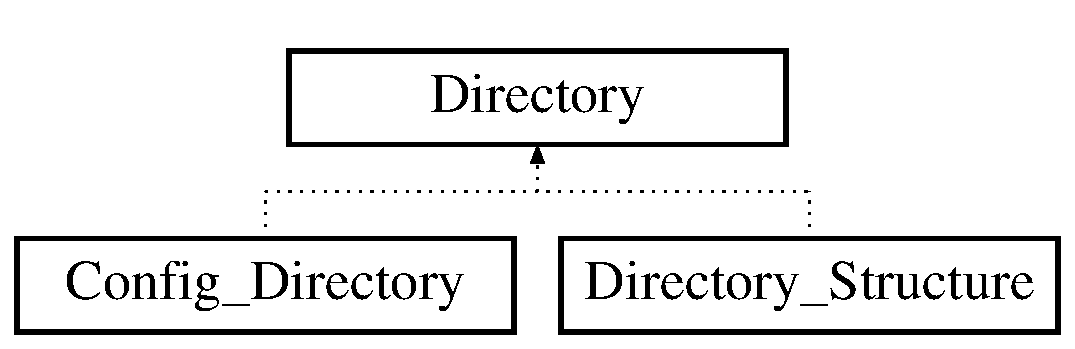
\includegraphics[height=2.000000cm]{class_directory}
\end{center}
\end{figure}
\subsection*{Public Member Functions}
\begin{DoxyCompactItemize}
\item 
\mbox{\Hypertarget{class_directory_a672adf44186f0a5b859681b858199060}\label{class_directory_a672adf44186f0a5b859681b858199060}} 
{\bfseries Directory} (const std\+::string \&)
\item 
\mbox{\Hypertarget{class_directory_a1e6c830b4852be463ee627eaf2f4851e}\label{class_directory_a1e6c830b4852be463ee627eaf2f4851e}} 
{\bfseries Directory} (const \mbox{\hyperlink{class_directory}{Directory}} \&)
\item 
\mbox{\Hypertarget{class_directory_aa34f63559f0f4df446619cc3f8feeb4a}\label{class_directory_aa34f63559f0f4df446619cc3f8feeb4a}} 
\mbox{\hyperlink{class_directory}{Directory}} \& {\bfseries operator=} (const std\+::string \&)
\item 
\mbox{\Hypertarget{class_directory_a83d6fc87791ff52071eabb7fd72c24fb}\label{class_directory_a83d6fc87791ff52071eabb7fd72c24fb}} 
\mbox{\hyperlink{class_directory}{Directory}} \& {\bfseries operator=} (const \mbox{\hyperlink{class_directory}{Directory}} \&)
\item 
\mbox{\Hypertarget{class_directory_ad219c1eb86a1359c28e7fbfe34c45232}\label{class_directory_ad219c1eb86a1359c28e7fbfe34c45232}} 
void \mbox{\hyperlink{class_directory_ad219c1eb86a1359c28e7fbfe34c45232}{set\+\_\+input}} (const std\+::string \&)
\begin{DoxyCompactList}\small\item\em change string on path and assign to directory out path \end{DoxyCompactList}\item 
\mbox{\Hypertarget{class_directory_a4cb94f24bee78cd0c1e50bad3f773b74}\label{class_directory_a4cb94f24bee78cd0c1e50bad3f773b74}} 
void {\bfseries copy} (const \mbox{\hyperlink{class_directory}{Directory}} \&)
\item 
\mbox{\Hypertarget{class_directory_a4c4d39af239f886cbbebae40b86d87db}\label{class_directory_a4c4d39af239f886cbbebae40b86d87db}} 
const std\+::string \mbox{\hyperlink{class_directory_a4c4d39af239f886cbbebae40b86d87db}{get\+\_\+directory}} ()
\begin{DoxyCompactList}\small\item\em return path.\+directory \end{DoxyCompactList}\item 
\mbox{\Hypertarget{class_directory_ac632fb50196d0cceab655863bbf69f18}\label{class_directory_ac632fb50196d0cceab655863bbf69f18}} 
const std\+::string \mbox{\hyperlink{class_directory_ac632fb50196d0cceab655863bbf69f18}{get\+\_\+filename}} ()
\begin{DoxyCompactList}\small\item\em return path.\+file \end{DoxyCompactList}\item 
\mbox{\Hypertarget{class_directory_a482645277603ef32cccc41d144ab2f4e}\label{class_directory_a482645277603ef32cccc41d144ab2f4e}} 
const std\+::string \mbox{\hyperlink{class_directory_a482645277603ef32cccc41d144ab2f4e}{get\+\_\+path}} ()
\begin{DoxyCompactList}\small\item\em return path.\+directory + path.\+file \end{DoxyCompactList}\item 
\mbox{\Hypertarget{class_directory_a5226980ca7e90c292032a04a308f812a}\label{class_directory_a5226980ca7e90c292032a04a308f812a}} 
const std\+::string \mbox{\hyperlink{class_directory_a5226980ca7e90c292032a04a308f812a}{get\+\_\+username}} ()
\begin{DoxyCompactList}\small\item\em return current username \end{DoxyCompactList}\end{DoxyCompactItemize}
\subsection*{Protected Member Functions}
\begin{DoxyCompactItemize}
\item 
\mbox{\Hypertarget{class_directory_a63681e65191b8c08c66bd8a5b01bd304}\label{class_directory_a63681e65191b8c08c66bd8a5b01bd304}} 
void {\bfseries clear} ()
\item 
\mbox{\Hypertarget{class_directory_a1f4dbc8eb485cd10226408ae0193d79f}\label{class_directory_a1f4dbc8eb485cd10226408ae0193d79f}} 
bool {\bfseries root} ()
\end{DoxyCompactItemize}
\subsection*{Protected Attributes}
\begin{DoxyCompactItemize}
\item 
\mbox{\Hypertarget{class_directory_a7a883ac4b3a81b11521af22a0f66a112}\label{class_directory_a7a883ac4b3a81b11521af22a0f66a112}} 
\begin{tabbing}
xx\=xx\=xx\=xx\=xx\=xx\=xx\=xx\=xx\=\kill
struct \{\\
\>boost::filesystem::path {\bfseries directory}\\
\>boost::filesystem::path {\bfseries file}\\
\} {\bfseries path}\\

\end{tabbing}\item 
\mbox{\Hypertarget{class_directory_afabc4c126084ec2539411a110c3fc922}\label{class_directory_afabc4c126084ec2539411a110c3fc922}} 
std\+::string {\bfseries username}
\end{DoxyCompactItemize}


\subsection{Detailed Description}
Manage directory and path. 

\mbox{\hyperlink{class_directory}{Directory}} contain directory our directory and filename. 

The documentation for this class was generated from the following files\+:\begin{DoxyCompactItemize}
\item 
include/directory.\+h\item 
src/directory.\+cpp\end{DoxyCompactItemize}

\hypertarget{class_directory___structure}{}\section{Directory\+\_\+\+Structure Class Reference}
\label{class_directory___structure}\index{Directory\+\_\+\+Structure@{Directory\+\_\+\+Structure}}
Inheritance diagram for Directory\+\_\+\+Structure\+:\begin{figure}[H]
\begin{center}
\leavevmode
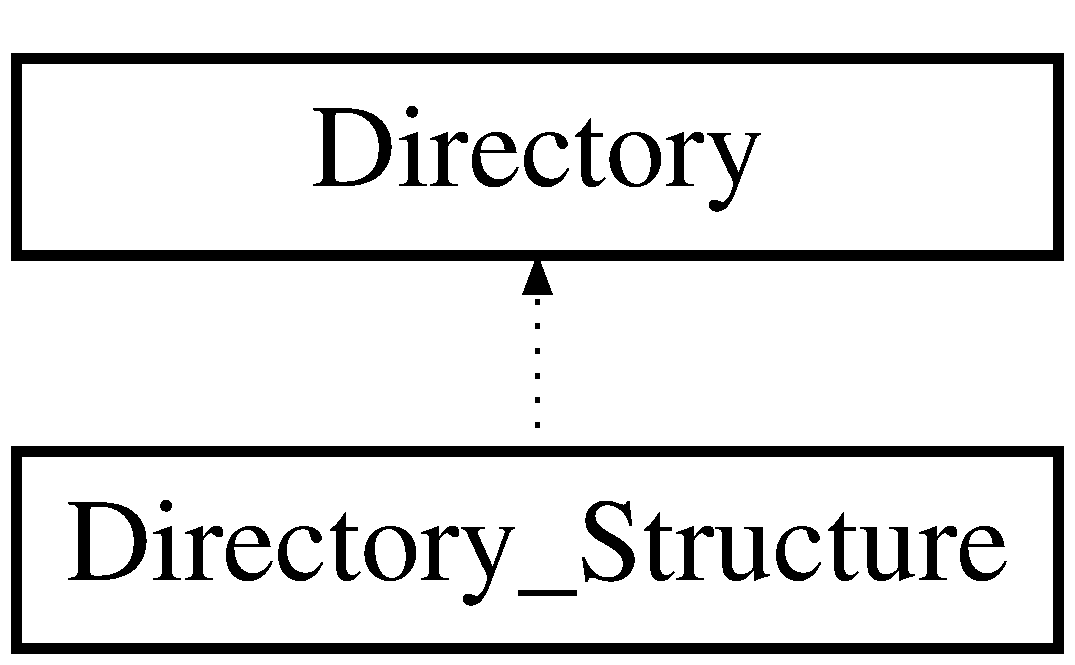
\includegraphics[height=2.000000cm]{class_directory___structure}
\end{center}
\end{figure}
\subsection*{Public Member Functions}
\begin{DoxyCompactItemize}
\item 
\mbox{\Hypertarget{class_directory___structure_ab8fc3a4c43a8368440260becd511f660}\label{class_directory___structure_ab8fc3a4c43a8368440260becd511f660}} 
{\bfseries Directory\+\_\+\+Structure} (const std\+::string \&)
\item 
\mbox{\Hypertarget{class_directory___structure_a9ebc08c7aea0df68cc3d7fdbecd3d32e}\label{class_directory___structure_a9ebc08c7aea0df68cc3d7fdbecd3d32e}} 
void {\bfseries map\+\_\+directory} (const std\+::string \&)
\end{DoxyCompactItemize}


The documentation for this class was generated from the following files\+:\begin{DoxyCompactItemize}
\item 
include/directory\+\_\+structure.\+h\item 
src/directory\+\_\+structure.\+cpp\end{DoxyCompactItemize}

\hypertarget{class_interface}{}\section{Interface Class Reference}
\label{class_interface}\index{Interface@{Interface}}
\subsection*{Public Types}
\begin{DoxyCompactItemize}
\item 
\mbox{\Hypertarget{class_interface_a30f9918f0087b9854d68be4eb2eee487}\label{class_interface_a30f9918f0087b9854d68be4eb2eee487}} 
enum {\bfseries F\+L\+A\+GS} \{ {\bfseries G\+L\+O\+B\+AL} = 0, 
{\bfseries T\+E\+XT} = 1
 \}
\end{DoxyCompactItemize}
\subsection*{Public Member Functions}
\begin{DoxyCompactItemize}
\item 
\mbox{\Hypertarget{class_interface_add0beb0b012e64d5bb6f94cecb1b01d8}\label{class_interface_add0beb0b012e64d5bb6f94cecb1b01d8}} 
virtual bool {\bfseries take\+\_\+directories} (const path \&)
\item 
\mbox{\Hypertarget{class_interface_a1049e20fb137ea850b2a3568c82b36e1}\label{class_interface_a1049e20fb137ea850b2a3568c82b36e1}} 
virtual bool {\bfseries take\+\_\+directories} (const std\+::vector$<$ path \&$>$)
\end{DoxyCompactItemize}


The documentation for this class was generated from the following file\+:\begin{DoxyCompactItemize}
\item 
include/interface.\+h\end{DoxyCompactItemize}

\hypertarget{class_main_window}{}\section{Main\+Window Class Reference}
\label{class_main_window}\index{Main\+Window@{Main\+Window}}
Inheritance diagram for Main\+Window\+:\begin{figure}[H]
\begin{center}
\leavevmode
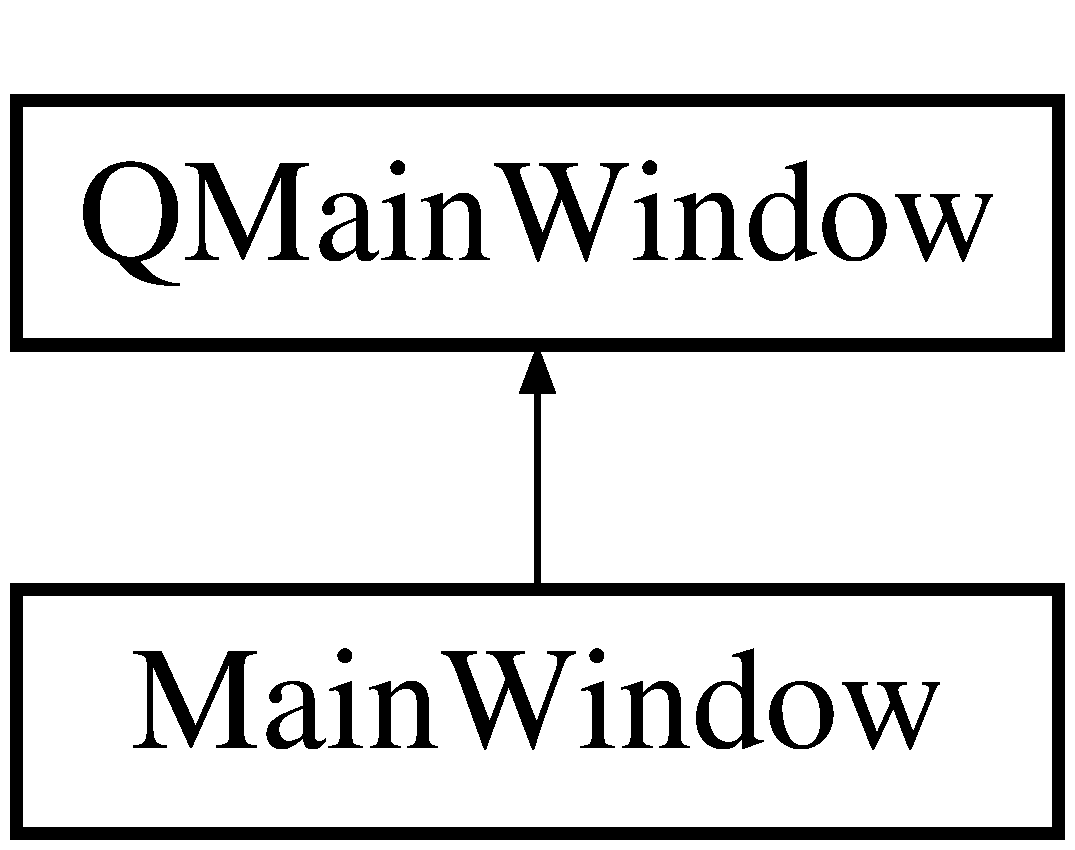
\includegraphics[height=2.000000cm]{class_main_window}
\end{center}
\end{figure}
\subsection*{Public Member Functions}
\begin{DoxyCompactItemize}
\item 
\mbox{\Hypertarget{class_main_window_a996c5a2b6f77944776856f08ec30858d}\label{class_main_window_a996c5a2b6f77944776856f08ec30858d}} 
{\bfseries Main\+Window} (Q\+Widget $\ast$parent=nullptr)
\end{DoxyCompactItemize}


The documentation for this class was generated from the following files\+:\begin{DoxyCompactItemize}
\item 
G\+U\+I/mainwindow.\+h\item 
G\+U\+I/mainwindow.\+cpp\end{DoxyCompactItemize}

%--- End generated contents ---

% Index
\backmatter
\newpage
\phantomsection
\clearemptydoublepage
\addcontentsline{toc}{chapter}{Index}
\printindex

\end{document}
